\section*{Appendix A - General} \label{append:a}
Link to the Ethics form and Participant Information Sheet:

\url{https://falmouthac-my.sharepoint.com/:f:/g/personal/to231922_falmouth_ac_uk/EiE3vOcxqLlLuU0_BN7m1NoBCja231kbqKHAxOlqX-sRfw?e=4dc65R}
\\
\\
Link to the Computing Artefact GitHub repository: 
\url{https://github.com/thomasoleary/dissertation-artefact.git}
\begin{figure}[ht]
    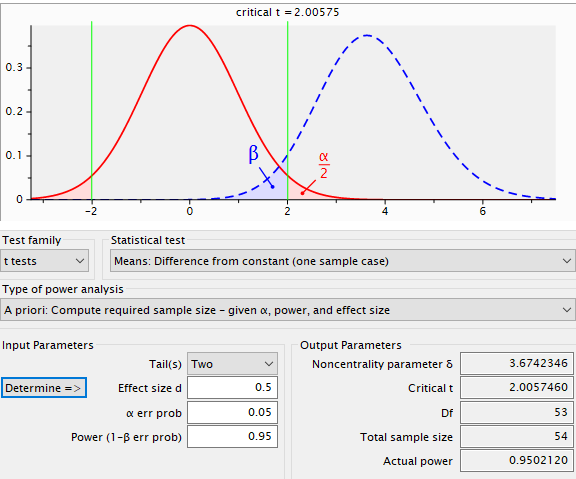
\includegraphics[width=\columnwidth]{./Images/gpower.png}
    \centering
    \caption{G*Power Sample Size}
    \label{gpower}
\end{figure}

\newpage
\section*{Appendix B - Reflective Addendum} \label{append:b}
\subsubsection{Lost ambition for Game Development}
Around midway through the first study block in my second year of study at Falmouth University - I lost my ambition for game development and the drive to want to become a game programmer in the industry. This loss of ambition almost drove me to dropping out of my studies at Falmouth and to look for an appropriate course to continue my studies elsewhere. Nonetheless, I persisted through as I believed that having only 1 more year to complete was better than restarting my studies. Losing my ambition towards game development has put a lot of weight on my shoulders with the work I do as I simply do not enjoy the modules I partake in as almost everything regarding Computing For Games BSc is game related. With this in mind, deciding what to do for my dissertation was a very difficult decision as I did not want to end up researching into a topic that was heavily game based. Ultimately, I feel that I found a topic that I deemed interesting enough to explore as it was quite minimally game based - but also something that I could see through to the end without having the consideration of changing ideas.
\\
\subsubsection{Motivation towards Project}
As the second study block began for my final year, I began to feel a lot more invested in completing anything but my tasks for my dissertation. I found myself spending most days completing my tasks for my team's GAM330 project (Multi-disciplinary group project). I realised that this became a real issue around Week 3 of Study Block 2 (SB2) but didn't do anything to adjust/fix the issue until Week 6. Once I stuck my head down and started churning away at my tasks, I soon realised that I found managing individual projects very difficult. I tended to get all of my tasks stuck in my head and end up getting distracted and/or lost very easily by focusing on something irrelevant/menial. I feel that one way that could've helped ease these issues of project management was by communicating with my project supervisor much more frequently with how I felt about my dissertation's progress. Furthermore, I may have benefited from the advice that they would give regarding how I was dealing with my work load.
\\
\subsubsection{Unit Testing}
Whilst developing my Artefact, I found Unit Testing a difficult task to continuously follow. For starters, whilst developing my artefact it was my first time that I had personally used Unit Tests to validate my code. After finishing my studies at Falmouth University, I strive to enter the world of Software Engineering and hopefully land a job as a developer. But with this, Unit Tests must become the norm for me when it comes to validating my work. I believe I should begin to write code with Unit Tests already in mind or perhaps take up the strict style of writing Unit Tests before proceeding with coding.

\newpage
Not-so-SMART Objective: Unit Test more often
\\
\begin{tabular}{| p{0.3\columnwidth} | p{0.5\columnwidth} |}
    \hline
    \textbf{Key Component} & \textbf{Objective} \\
    \hline
    Specific & I aim to use Unit Tests more to validate my work.\\
    \hline
    Measurable & By planning and writing tests before completing a task.\\
    \hline
    Achievable & This is achievable as I have base knowledge on writing Unit Tests to validate my work.\\
    \hline
    Realistic & This is realistic as there are online resources to help and the assistance by others.\\
    \hline
    Time-Bound & This will be completed for the next personal project I will complete within 3 months.\\
    \hline
\end{tabular}
\\
SMART Object: For the remainder of my time at University, I would like to improve on Unit Testing to validate my work by planning and writing tests before proceeding with code. I will do this through the use of online resources and the assistance of others.

\newpage
\section*{Appendix C - Software Architecture} \label{append:c}
\begin{figure}[!h]
    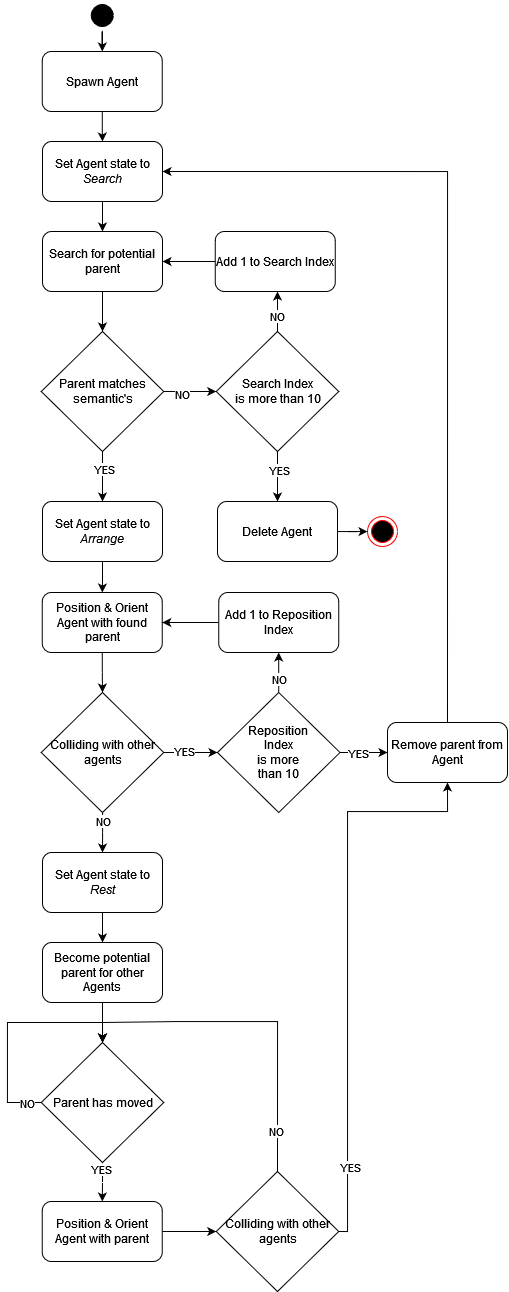
\includegraphics[width=\columnwidth]{./Images/AgentActivityDiagram.png}
    \centering
    \caption{Agent Behaviour represented in an Activity Diagram}
    \label{activity-diagram}
\end{figure}

\newpage
\section*{Appendix D - Testing} \label{append:d}
The Unit tests for my artefact were created using Unity's Test Framework and were used throughout the Artefact's development to validate the code and to ensure the Artefact worked as intended. Unit testing code can be seen in \hyperref[append:f]{Appendix F} and passed Unit Tests can be seen in Fig~\ref{unit-tests}.
\\
A small pilot study was conducted with the help of some BSc peers. This pilot study was conducted to ensure the validity of my experimental design. It consisted of them taking part in my 2-staged A/B test, helping in testing the effectiveness of how information was being represented - any feedback received from this small study was implemented into my methodology and no data from this pilot study was used within my data analysis.

\begin{figure}[ht]
    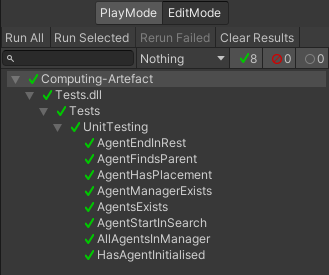
\includegraphics[width=\columnwidth]{./Images/unit-tests.png}
    \centering
    \caption{Unit Tests in the Unity Test Runner}
    \label{unit-tests}
\end{figure}

\newpage
\newpage
\section*{Appendix E - R Code} \label{append:e}
\lstinputlisting[language=r, label=StageOneRCode,caption=R Code for Stage One data., captionpos=b]{Code/StageOneRCode.R}

\lstinputlisting[language=r, label=StageTwoRCode,caption=R Code for Stage Two data., captionpos=b]{Code/StageTwoRCode.R}

\newpage
\section*{Appendix F - Unit Testing Code} \label{append:f}
\lstinputlisting[language=csh, label=UnitTestCode, caption=Unit Test Code used to validate the Artefact's code., captionpos =b]{Code/UnitTesting.cs}